% Property / insurance IoT -- internal engineering roadmap
% Build: make slides   (pdflatex twice; latexmk is not packaged on this box)
%
% DEPENDENCIES, deliberately minimal. This deck loads only:
%   beamer, pgf/tikz, booktabs, colortbl, xcolor, array, microtype
% and probes for sourcesanspro/helvet at build time. pgfplots, multirow,
% makecell, adjustbox, tcolorbox, pgfgantt, inconsolata and the Metropolis
% theme were all absent from the build box at some point during authoring, so
% nothing here requires them. The Gantt on slide 21 is plain TikZ primitives.
%
% xcolor options MUST go through \documentclass: beamer loads xcolor itself,
% so \usepackage[table]{xcolor} later throws an option clash. "table" is what
% gives us \cellcolor.
\documentclass[aspectratio=169,t,10pt,xcolor={table,svgnames}]{beamer}

\usepackage[T1]{fontenc}
\usepackage{booktabs}
\usepackage{colortbl}
\usepackage{array}
\usepackage{tikz}
\usepackage{microtype}

% Optional nicety: a real sans instead of Computer Modern Sans. Degrades
% gracefully so the deck still builds on a minimal TeX install.
%
% Note the ly1enc.def test: sourcesanspro.sty can be present while the LY1
% encoding it loads (texlive-ly1) is not, which fails the build with a
% confusing "Encoding file `ly1enc.def' not found". Probing for the .sty alone
% is not enough -- test the dependency that actually breaks.
\IfFileExists{ly1enc.def}{%
  \IfFileExists{sourcesanspro.sty}{\usepackage[default,scale=0.95]{sourcesanspro}}{}}{%
  \IfFileExists{helvet.sty}{\usepackage{helvet}\renewcommand{\familydefault}{\sfdefault}}{}}
\usefonttheme{professionalfonts}

% ---------------------------------------------------------------- palette
% Monotone greys with black text throughout. Contrast ratios vs black were
% computed, not eyeballed. Three fill levels plus empty is the maximum that
% survives laser halftoning, so every shaded cell ALSO carries a text token --
% the fill is redundant reinforcement, never the primary encoding.
\definecolor{fill0}{gray}{1.00}   % #ffffff  21.0:1  not started
\definecolor{fill1}{gray}{0.86}   % #dbdbdb  15.2:1
\definecolor{fill2}{gray}{0.68}   % #adadad   9.4:1
\definecolor{fill3}{gray}{0.46}   % #757575   4.6:1  darkest fill keeping black text
\definecolor{ink}{gray}{0.12}
\definecolor{inkmute}{gray}{0.42}
\definecolor{hair}{gray}{0.72}
\definecolor{accent}{HTML}{1F4E79} % structure only, NEVER data
%
% No red/amber/green anywhere. Verified: status green #0ca30c prints as
% gray 0.55 and status red #d03b3b as gray 0.45 -- about 1.3:1 apart in
% greyscale, i.e. indistinguishable. Likelihood and impact are H/M/L text
% tokens and rows are sorted by L x I instead.

% ------------------------------------------------------------------ theme
% ~30 lines on `default` rather than a packaged theme. Flat square blocks are
% what actually stop a deck reading as 2009; the rounded drop-shadow block is
% the tell.
\usetheme{default}
\useinnertheme{rectangles}
\setbeamertemplate{blocks}[default]
\setbeamertemplate{navigation symbols}{}
\setbeamersize{text margin left=7mm,text margin right=7mm}
\setbeamercolor{normal text}{fg=ink}
\setbeamercolor{frametitle}{fg=ink}
\setbeamercolor{structure}{fg=accent}
\setbeamercolor{itemize item}{fg=inkmute}
\setbeamercolor{itemize subitem}{fg=inkmute}
\setbeamertemplate{itemize item}{\raisebox{0.15ex}{\scriptsize$\blacksquare$}}
\setbeamertemplate{itemize subitem}{\raisebox{0.15ex}{\tiny$\square$}}
\setbeamerfont{frametitle}{size=\large,series=\bfseries}

% Left-aligned sentence-case frame title with a thin rule beneath.
\setbeamertemplate{frametitle}{%
  \vspace{2.2ex}%
  \begin{minipage}{\dimexpr\paperwidth-14mm\relax}%
    \raggedright\usebeamerfont{frametitle}\usebeamercolor[fg]{frametitle}\insertframetitle%
    \par\vspace{0.6ex}{\color{hair}\hrule height 0.6pt}%
  \end{minipage}\par\vspace{0.4ex}}

\setbeamertemplate{footline}{%
  \hbox{\begin{beamercolorbox}[wd=\paperwidth,ht=3ex,dp=1.6ex,leftskip=7mm,rightskip=7mm]{}%
    {\color{inkmute}\scriptsize\insertshorttitle\hfill\insertframenumber\,/\,\inserttotalframenumber}%
  \end{beamercolorbox}}}

% ------------------------------------------------------------- shorthands
\newcommand{\gate}[1]{%
  \begin{beamercolorbox}[wd=\textwidth,sep=1.6ex]{}%
    \color{ink}\small\textbf{Exit gate.}\, #1%
  \end{beamercolorbox}}
\newcommand{\yes}{\textbf{Y}}
\newcommand{\no}{--}
\newcommand{\hd}[1]{\textbf{\footnotesize #1}}
% Gantt bar for slide 21: {row y}{x start}{x end}{fill}{label}.
%
% MUST be defined in the preamble, not inside the tikzpicture: \newcommand with
% # parameters inside a picture that also uses \foreach collides with PGF's
% internal \iterate and fails with "Illegal parameter number in definition of
% \iterate".
%
% Task names go in a fixed LEFT GUTTER rather than beside the bar. Labels placed
% at the bar's right end overlap each other and the grid as soon as two short
% bars land in adjacent months, which is exactly what the real schedule does.
\newcommand{\gbar}[5]{%
  \fill[#4] (#2,#1+0.28) rectangle (#3,#1-0.28);
  \draw[hair,line width=0.4pt] (#2,#1+0.28) rectangle (#3,#1-0.28);
  \node[anchor=east,font=\tiny,align=right,text width=3.1cm] at (-0.7,#1) {#5};}

% build/use/partner tokens
\newcommand{\tB}{\cellcolor{fill3}\textbf{B}}
\newcommand{\tU}{\cellcolor{fill1}U}
\newcommand{\tP}{\cellcolor{fill2}P}
\newcommand{\tN}{\cellcolor{fill0}\textcolor{inkmute}{--}}

\title{Property IoT for Insurance Perils}
\subtitle{Internal engineering roadmap}
\date{14 October 2026}
\begin{document}

% ============================================================= 1
\begin{frame}[plain]
  \vspace{1.2cm}
  {\LARGE\bfseries Property IoT for Insurance Perils\par}
  \vspace{0.3cm}
  {\large\color{inkmute} Internal engineering roadmap \textperiodcentered{} North America\par}
  \vspace{0.9cm}
  {\footnotesize
   Escape of water \textperiodcentered{} electrical fire precursors\\
   LoRaWAN US915 \textperiodcentered{} BLE \textperiodcentered{} Thread/Matter \textperiodcentered{} LTE-M\par}
  \vspace{0.7cm}
  {\scriptsize\color{inkmute}
   14 October 2026 \textperiodcentered{} \textbf{This is not an investor deck.}
   No market-size slide. Figures marked [V] are vendor-published; [E] are estimates.\par}
\end{frame}

% ============================================================= 2
\begin{frame}{What this deck decides}
  \small
  \begin{tabular}{@{}p{0.30\textwidth}p{0.40\textwidth}p{0.22\textwidth}@{}}
    \toprule
    \hd{Decision} & \hd{Options} & \hd{Decide by} \\
    \midrule
    Module ecosystem & RAK/Nordic/Espressif on one SDK & \textbf{Week 1} \\
    Radio            & LoRaWAN \textperiodcentered{} BLE \textperiodcentered{} LTE-M \textperiodcentered{} Thread & Week 6 (P0 gate) \\
    Shutoff story    & Resell certified \textperiodcentered{} retrofit actuator \textperiodcentered{} advisory only & Week 6 (P0 gate) \\
    Build model      & Own-design \textperiodcentered{} ODM rebadge \textperiodcentered{} licence \textperiodcentered{} software & Month 5 (P2) \\
    \bottomrule
  \end{tabular}
  \vspace{0.6em}
  \begin{itemize}\footnotesize
    \item Week-1 decision is the \emph{ecosystem}, not the radio. Radio is downstream of the buyer.
    \item Everything else in year 1 is cheap to reverse. The module choice is not.
  \end{itemize}
\end{frame}

% ============================================================= 3
\begin{frame}{The constraint}
  \begin{itemize}
    \item \textbf{\$25k--\$100k non-salary} for the first 12 months.
    \item \textbf{Full in-house EE} --- schematic, PCB, RF, enclosure.
  \end{itemize}
  \vspace{0.5em}
  {\color{hair}\hrule height 0.6pt}
  \vspace{0.5em}
  \begin{itemize}
    \item So design labour costs \textbf{calendar}, not cash.
    \item What costs cash: \textbf{test labs, listings, tooling, parts, lab time} --- and none of it
          gets cheaper because the layout is good.
  \end{itemize}
  \vspace{0.8em}
  \begin{beamercolorbox}[wd=\textwidth,sep=1.6ex]{}
    \color{ink}\small Certification is a \textbf{\$20--60k} problem.\\
    The company-ending problems are \textbf{nobody will sign} and \textbf{a winter of data cannot be bought}.
  \end{beamercolorbox}
\end{frame}

% ============================================================= 4
\begin{frame}{The two gates that set cost}
  \centering
  \begin{tikzpicture}[font=\footnotesize]
    % axes labels
    \node[anchor=south,align=center] at (3.6,3.5) {\textbf{Mains voltage inside the enclosure?}};
    \node[anchor=south] at (1.7,3.0) {no};
    \node[anchor=south] at (5.5,3.0) {yes};
    \node[rotate=90,anchor=south,align=center] at (-1.5,1.2)
      {\textbf{Wetted surface in the BOM?}};
    \node[anchor=east] at (-0.6,2.1) {no};
    \node[anchor=east] at (-0.6,0.3) {yes};
    % cells
    \fill[fill0] (-0.2,1.2) rectangle (3.6,3.0);
    \draw[hair,line width=0.6pt] (-0.2,1.2) rectangle (3.6,3.0);
    \node[align=center,text width=3.4cm] at (1.7,2.1)
      {\textbf{A, B, C}\\ FCC Part 15 only\\[0.2em] \textbf{\$31--94k}};
    \fill[fill2] (3.6,1.2) rectangle (7.4,3.0);
    \draw[hair,line width=0.6pt] (3.6,1.2) rectangle (7.4,3.0);
    \node[align=center,text width=3.4cm] at (5.5,2.1)
      {\textbf{D} plug-in detector\\ $+$ NRTL: UL 498, 60730-1, 94\\[0.2em] \textbf{\$180--560k}};
    \fill[fill1] (-0.2,-0.6) rectangle (3.6,1.2);
    \draw[hair,line width=0.6pt] (-0.2,-0.6) rectangle (3.6,1.2);
    \node[align=center,text width=3.4cm] at (1.7,0.3)
      {sub-metering\\ $+$ NSF 61 \& 372};
    \fill[fill3] (3.6,-0.6) rectangle (7.4,1.2);
    \draw[hair,line width=0.6pt] (3.6,-0.6) rectangle (7.4,1.2);
    \node[align=center,text width=3.4cm] at (5.5,0.3)
      {\textbf{E} inline valve\\ $+$ IGC 115/349 $+$ NSF\\ $+$ cUPC \textperiodcentered{} \textbf{\$112--366k}};
    % annotation
    \node[anchor=west,align=left,text width=4.6cm,font=\scriptsize] at (7.8,2.1)
      {Cross \emph{right}: $+$\$15--40k NRTL, plus annual factory inspections.\\[0.4em]
       Cross \emph{down}: $+$\$25--80k plumbing listing, plus a licensed plumber to install.};
  \end{tikzpicture}
  \vspace{0.4em}
  {\scriptsize\color{inkmute} All eight ``start now'' applications avoid both gates. That quadrant
   is the portfolio.\par}
\end{frame}

% ============================================================= 5
\begin{frame}{Five options, re-cut on the gates}
  \scriptsize
  \begin{tabular}{@{}p{0.27\textwidth}cccp{0.19\textwidth}c@{}}
    \toprule
    \hd{Option} & \hd{Mains} & \hd{Wetted} & \hd{Cash [E]} & \hd{Gates} & \hd{Year 1?} \\
    \midrule
    A. Clamp-on leak sensor (battery)   & \no  & \no  & \textbf{\$31--94k}  & FCC Part 15            & \cellcolor{fill1}\textbf{Yes} \\
    B. Retrofit lever actuator          & \no  & \no  & \$70--231k          & FCC; IAPMO likely N/A  & \cellcolor{fill1}\textbf{Spike} \\
    C. Gateway on a listed adapter      & \no  & \no  & low                 & FCC 15B/15C            & \cellcolor{fill1}\textbf{Yes} \\
    D. Plug-in electrical detector      & \yes & \no  & \$180--560k         & $+$ UL 498, 60730-1, 94 & \cellcolor{fill2}No \\
    E. Inline motorised valve           & \yes & \yes & \$112--366k         & $+$ IGC, NSF, cUPC     & \cellcolor{fill2}No \\
    \bottomrule
  \end{tabular}
  \vspace{0.8em}
  \begin{itemize}\footnotesize
    \item \textbf{B dodges the plumbing standards} --- an external bracket has no wetted surface and
          no pressure boundary. The blocker is \emph{mechanical}, not regulatory.
    \item Ship the shutoff story on a \textbf{third-party certified valve} in year 1.
  \end{itemize}
\end{frame}

% ============================================================= 6
\begin{frame}{What is actually on the critical path}
  \begin{itemize}
    \item \textbf{Not hardware.}
    \item buyer signature $\rightarrow$ installed base $\rightarrow$ \textbf{one freeze/thaw cycle of
          labelled data} $\rightarrow$ defensible nuisance rate $\rightarrow$ security review
          $\rightarrow$ filing.
    \item FCC and PCB sit on a \emph{parallel} path that must merely not be late.
    \item The one non-compressible item is \textbf{calendar time in the field across a winter}.
          Cash cannot buy it; parallelism cannot shorten it.
  \end{itemize}
  \vspace{0.6em}
  \begin{beamercolorbox}[wd=\textwidth,sep=1.6ex]{}
    \color{ink}\small \textbf{Standing rule 1: no PCB layout in the first 90 days.}\\
    Free design labour is a trap. It spends calendar --- the only unbuyable resource ---
    on a board nobody can yet validate. \textbf{Miss October and you slip a year, not a quarter.}
  \end{beamercolorbox}
\end{frame}

% ============================================================= 7
\begin{frame}{The spine: P0--P4, one hard gate each}
  \scriptsize
  \begin{tabular}{@{}p{0.15\textwidth}p{0.08\textwidth}p{0.10\textwidth}p{0.55\textwidth}@{}}
    \toprule
    \hd{Phase} & \hd{Window} & \hd{Cash [E]} & \hd{The single exit gate} \\
    \midrule
    \textbf{P0} Falsify the buyer & wk 0--6  & \$6--14k  & A \textbf{countersigned} paid pilot or LOI for $\geq$50 units \emph{with a start date} \\
    \textbf{P1} Prove the alert   & wk 6--20 & \$12--28k & \textbf{$<$0.5 nuisance alerts/device-year} over $\geq$90 days on $\geq$50 devices, frozen eval set, $\geq$1 true event \\
    \textbf{P2} Own the node      & mo 5--12 & \$25--55k & \textbf{FCC grant in hand}; first run at landed cost $\leq$60\% of contracted price \\
    \rowcolor{fill1}
    \textbf{P3} Mains \& water    & mo 12--24& \textbf{\$150--400k} & Signed MSA $+$ $\geq$1 state rate/rule filing in progress \\
    \rowcolor{fill1}
    \textbf{P4} Risk data product & mo 24--36& \textbf{raise}       & An \emph{approved} filing, or renewal at measurable price uplift \\
    \bottomrule
  \end{tabular}
  \vspace{0.7em}
  \begin{itemize}\footnotesize
    \item P0--P2 total \textbf{\$43--97k} --- inside the envelope, \emph{if} the first production run
          is PO-funded.
    \item Shaded rows \textbf{require a raise}. P3 alone is 2--4$\times$ the entire year-1 budget.
  \end{itemize}
\end{frame}

% ============================================================= 8
\begin{frame}{Layer $\times$ phase, layers 1--5}
  \scriptsize
  \begin{tabular}{@{}p{0.17\textwidth}p{0.14\textwidth}p{0.16\textwidth}p{0.16\textwidth}p{0.15\textwidth}p{0.13\textwidth}@{}}
    \toprule
    \hd{Layer} & \hd{P0} & \hd{P1} & \hd{P2} & \hd{P3} & \hd{P4} \\
    \midrule
    Sensing            & 2$\times$TMP117 on kit & ODM sensors    & \cellcolor{fill1}own PCB      & $+$mains/wetted  & multi-peril \\
    Edge compute/ML    & \cellcolor{fill0}none  & \cellcolor{fill0}none (cloud) & CMSIS-DSP      & emlearn on-device& on-device anomaly \\
    Radio \& WAN       & LoRaWAN bench          & \cellcolor{fill1}buyer decides& one family, 2nd-src & $+$Matter   & $+$Sidewalk eval \\
    Device mgmt \& OTA & \cellcolor{fill0}none  & Golioth trial  & \cellcolor{fill1}MCUboot $+$ mcumgr/BLE & staged $+$ canary & fleet SLA \\
    Cloud \& data      & ingest $+$ raw retention & TTS, VerneMQ, IoTDB & Magistrala $+$ RBAC & multi-tenant portal & warehouse \\
    \bottomrule
  \end{tabular}
  \vspace{0.7em}
  \begin{itemize}\footnotesize
    \item \textbf{No neural network on the node before P2.} You cannot compress a model you have not
          trained on data you do not have.
    \item \textbf{Raw retention from day one.} The corpus is the only asset cash cannot compress.
  \end{itemize}
\end{frame}

% ============================================================= 9
\begin{frame}{Layer $\times$ phase, layers 6--9}
  \scriptsize
  \begin{tabular}{@{}p{0.19\textwidth}p{0.17\textwidth}p{0.17\textwidth}p{0.14\textwidth}p{0.13\textwidth}p{0.11\textwidth}@{}}
    \toprule
    \hd{Layer} & \hd{P0} & \hd{P1} & \hd{P2} & \hd{P3} & \hd{P4} \\
    \midrule
    Analytics \& risk model & hand-labelled & \cellcolor{fill1}shadow classifier & tuned rejection & severity model & portfolio score \\
    \textbf{Who signs the paper} & 25 convos, 4 routes & \cellcolor{fill3}\textbf{1 countersigned} & aggregator & carrier MSA & $+$reinsurer \\
    Compliance \& cert & \cellcolor{fill1}IAPMO scope letter & E\&O; SOC 2 I & \cellcolor{fill3}\textbf{FCC grant} & NRTL, IGC, NSF & SOC 2 II \\
    Field ops \& support & you install & install-verify telemetry & installer web app & dispatch SLA & regional partners \\
    \bottomrule
  \end{tabular}
  \vspace{0.7em}
  \begin{itemize}\footnotesize
    \item \textbf{``Who signs the paper'' is a technology layer here}, not a sales footnote --- it is
          the most likely single cause of death.
    \item Analytics is the only layer that is \emph{actually the product}.
  \end{itemize}
\end{frame}

% ============================================================= 10
\begin{frame}{Build / use / partner, per layer}
  \scriptsize
  \begin{tabular}{@{}p{0.20\textwidth}cccc p{0.42\textwidth}@{}}
    \toprule
    \hd{Layer} & \hd{P0} & \hd{P1} & \hd{P2} & \hd{P3} & \hd{Why} \\
    \midrule
    Sensing              & \tU & \tU & \tB & \tB & Commodity until the clamp mechanics are yours \\
    Edge compute/ML      & \tN & \tN & \tU & \tB & No NN before P2 \\
    Radio \& WAN         & \tU & \tU & \tU & \tU & \textbf{Never build a radio.} Modular inheritance is worth \$10--25k/SKU \\
    Device mgmt \& OTA   & \tN & \tU & \tU & \tU & \textbf{Never build this.} Golioth is Apache-2.0 with PKI rotation \\
    Cloud \& data        & \tB & \tB & \tB & \tB & Cheap, and where carrier-facing differentiation lives \\
    Analytics \& risk    & \tB & \tB & \tB & \tB & \textbf{The only layer that is the product} \\
    Who signs the paper  & \tB & \tP & \tP & \tP & Pre-seed cannot clear carrier vendor qualification \\
    Compliance \& cert   & \tP & \tP & \tP & \tP & Labs and NRTLs, always \\
    Field ops \& support & \tB & \tB & \tP & \tP & Install quality decides your false-positive rate \\
    \bottomrule
  \end{tabular}
  \vspace{0.5em}
  {\scriptsize\color{inkmute}\textbf{B} build \textperiodcentered{} \textbf{U} use existing
   \textperiodcentered{} \textbf{P} partner \textperiodcentered{} \textbf{--} not yet.
   Shading reinforces the token; it does not replace it.\par}
\end{frame}

% ============================================================= 11
\begin{frame}{Sensing front ends: what each can discriminate}
  \scriptsize
  \begin{tabular}{@{}p{0.17\textwidth}p{0.26\textwidth}p{0.24\textwidth}p{0.24\textwidth}@{}}
    \toprule
    \hd{Modality} & \hd{Detects} & \hd{Cannot discriminate} & \hd{Parts [V]} \\
    \midrule
    \textbf{Thermal $\Delta$T} (clamp-on) & continuous draw anywhere on the main; claimed to 5\,ml/min & leak \emph{location}; a running appliance vs a leak without time context & 2$\times$ TMP117 \$3.62@1k \\
    Acoustic              & pipe-borne leak noise; bursts & HVAC, traffic, appliance noise without ML & TDK T5838 (\textbf{20\,\textmu A wake-on-sound}); SPH0645 \$1.45@1k \\
    Vibration             & structure-borne events & low-amplitude seepage & ST IIS3DWB \$13--15@1k --- \textbf{2--3$\times$ the radio} \\
    Flow (ultrasonic)     & true volume; $<$1\,L/h & nothing --- but it is a meter-class BOM & MSP430FR6047 \$9.25@1k \\
    Pressure decay        & leaks from pressure \emph{alone}, single sensor & needs fast sampling; a DSP claim not a sensor claim & ordinary transducer $+$ DSP \\
    \bottomrule
  \end{tabular}
  \vspace{0.6em}
  \begin{itemize}\footnotesize
    \item \textbf{Use two TMP117, not an NTC divider.} Self-heating and tolerance stack eat a small
          persistent $\Delta$T.
    \item The T5838's \textbf{20\,\textmu A acoustic activity detect} is what makes battery acoustic
          viable at all.
  \end{itemize}
\end{frame}

% ============================================================= 12
\begin{frame}{Edge compute budget}
  \scriptsize
  \begin{tabular}{@{}p{0.22\textwidth}p{0.14\textwidth}p{0.14\textwidth}p{0.42\textwidth}@{}}
    \toprule
    \hd{Approach} & \hd{Flash} & \hd{RAM} & \hd{Verdict} \\
    \midrule
    CMSIS-DSP features only      & $<$10\,kB & $<$2\,kB & \cellcolor{fill1}\textbf{P0--P2.} FFT/MFCC/filters serve water \emph{and} electrical \\
    emlearn random forest        & \textbf{from 2\,kB} & \textbf{from 50\,B} & \cellcolor{fill1}\textbf{P2.} Built-in anomaly detection; MIT \\
    Microchip arc baseline       & 4--6\,kB & 1--2\,kB & 4 features, 160-sample windows @16\,kHz. \emph{Proprietary --- read, reimplement clean-room} \\
    tflite-micro $+$ CMSIS-NN    & 50--250\,kB & 20--60\,kB & P3. Only once the nuisance rate is known \\
    \bottomrule
  \end{tabular}
  \vspace{0.7em}
  \begin{beamercolorbox}[wd=\textwidth,sep=1.6ex]{}
    \color{ink}\small On a coin cell, \textbf{a 2\,kB forest that runs for five years beats a 200\,kB
    CNN that runs for eight months.}\\
    \textbf{LiteRT is not the MCU successor to TF Lite} --- it has no microcontroller support. Stay on
    \texttt{tflite-micro}.
  \end{beamercolorbox}
\end{frame}

% ============================================================= 13
\begin{frame}{Radio decision matrix}
  \scriptsize
  \begin{tabular}{@{}p{0.20\textwidth}ccccc@{}}
    \toprule
    \hd{Criterion} & \hd{LoRaWAN} & \hd{BLE} & \hd{Thread/Matter} & \hd{LTE-M} & \hd{Wi-Fi} \\
    \midrule
    Infrastructure you supply   & gateway        & phone/hub & border router & \cellcolor{fill1}\textbf{none} & none \\
    Works day one, no setup     & \no            & \no       & \no           & \cellcolor{fill1}\yes & \no \\
    Needs customer Wi-Fi creds  & \no            & \no       & yes           & \cellcolor{fill1}\no  & yes \\
    Battery life (sensor duty)  & \cellcolor{fill1}5--10\,yr & 2--5\,yr & 1--3\,yr & 2--5\,yr & months \\
    Basement/crawlspace reach   & \cellcolor{fill1}good      & poor--mod & poor--mod & good & poor \\
    Recurring \$/device         & \textasciitilde0 & 0 & 0 & \$1--3/yr & 0 \\
    \textbf{Downlink for shutoff} & \cellcolor{fill3}\textbf{bad} & good & good & moderate & good \\
    Consumer ecosystem          & none           & moderate  & \cellcolor{fill1}\textbf{Apple/Google/Amazon} & none & moderate \\
    Cert adder                  & \$3k$+$\$1.2k  & --        & \$10.5k       & PTCRB & -- \\
    \bottomrule
  \end{tabular}
  \vspace{0.6em}
  {\footnotesize \textbf{No single right radio. Segment by buyer:} multifamily $\rightarrow$ LoRaWAN
   $+$ building gateway \textperiodcentered{} carrier-mailed single-family $\rightarrow$ LTE-M
   \textperiodcentered{} DTC $\rightarrow$ BLE/Matter \textperiodcentered{} mains $\rightarrow$
   Wi-Fi/Thread.\par}
\end{frame}

% ============================================================= 14
\begin{frame}{The downlink problem}
  \scriptsize
  \begin{tabular}{@{}p{0.12\textwidth}p{0.36\textwidth}p{0.44\textwidth}@{}}
    \toprule
    \hd{Class} & \hd{Downlink behaviour} & \hd{Consequence for a shutoff command} \\
    \midrule
    \textbf{A} & Receive window opens \emph{only} after an uplink & \cellcolor{fill2}At a 15-min heartbeat, worst case is \textbf{15 minutes of flooding}. Unusable \\
    \textbf{B} & Scheduled ping slots on gateway beacons & Seconds, but beacon tracking burns power continuously \\
    \textbf{C} & Receive window open \textasciitilde continuously & Latency fine, \textbf{power budget gone} --- effectively mains \\
    \bottomrule
  \end{tabular}
  \vspace{0.9em}
  \begin{center}
  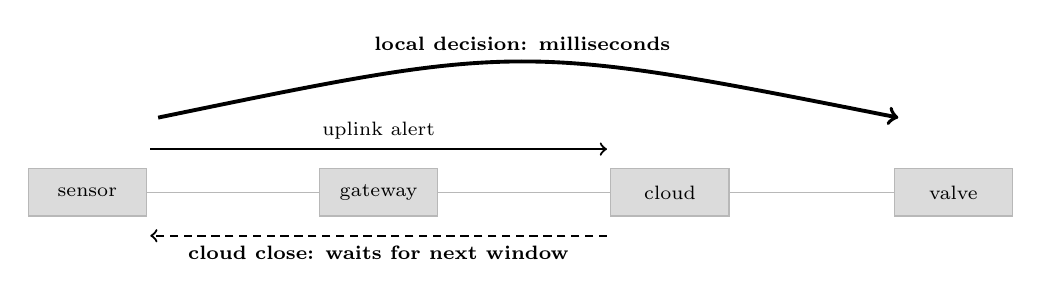
\begin{tikzpicture}[font=\scriptsize]
    \draw[hair,line width=0.5pt] (0,0) -- (11,0);
    \foreach \x/\l in {0/sensor,3.7/gateway,7.4/cloud,11/valve}
      {\fill[fill1] (\x-0.75,-0.3) rectangle (\x+0.75,0.3);
       \draw[hair] (\x-0.75,-0.3) rectangle (\x+0.75,0.3);
       \node at (\x,0) {\l};}
    \draw[->,line width=0.8pt] (0.8,0.55) -- node[above]{uplink alert} (6.6,0.55);
    \draw[->,line width=0.8pt,densely dashed] (6.6,-0.55) -- node[below]{\textbf{cloud close: waits for next window}} (0.8,-0.55);
    \draw[->,line width=1.4pt] (0.9,0.95) .. controls (5.5,1.9) .. node[above,pos=0.5]{\textbf{local decision: milliseconds}} (10.3,0.95);
  \end{tikzpicture}
  \end{center}
  \vspace{0.3em}
  \begin{beamercolorbox}[wd=\textwidth,sep=1.4ex]{}
    \color{ink}\small \textbf{Architectural, not operational: never put the shutoff decision on the
    WAN.} LoRaWAN carries alerts uplink. The close is decided locally or inside the valve; the cloud
    confirms and reports.
  \end{beamercolorbox}
\end{frame}

% ============================================================= 15
\begin{frame}{Power and battery arithmetic}
  \small
  \begin{itemize}
    \item \textbf{Li-SOCl\textsubscript{2} with a hybrid-layer capacitor. Never coin cells} for the
          main SKU --- Li-SOCl\textsubscript{2} cannot serve the TX pulse alone.
    \item \textbf{Derate datasheet capacity by \textasciitilde40\% for a cold basement}, and
          \emph{measure} pulse behaviour at $-10$ to $0^{\circ}$C rather than modelling it.
    \item Benchmarks to beat [V]: Milesight EM300-SLD \textbf{$>$10\,yr at SF7 US915};
          WS303 \textbf{\textasciitilde5.7\,yr} on a CR2450 590\,mAh.
  \end{itemize}
  \vspace{0.5em}
  {\color{hair}\hrule height 0.6pt}
  \vspace{0.5em}
  \begin{itemize}
    \item \textbf{Valve actuation is the power cliff.} Moen's Flo --- the market leader --- requires a
          nearby AC outlet and sells a 25-ft extension rather than going battery.
    \item So: \textbf{battery-only shutoff requires a latching solenoid, not a motor.} A
          tens-of-ms pulse holding state at zero standing current is the only topology that gets
          years on cells.
    \item \textbf{Fail-as-is, never fail-closed.} A valve that closes on battery death causes the
          freeze damage you were hired to prevent. Latching is inherently fail-as-is. Mechanical
          override on every unit.
  \end{itemize}
\end{frame}

% ============================================================= 16
\begin{frame}{Dev kit $\rightarrow$ production module}
  \scriptsize
  \begin{tabular}{@{}p{0.16\textwidth}p{0.17\textwidth}p{0.17\textwidth}p{0.15\textwidth}cp{0.14\textwidth}@{}}
    \toprule
    \hd{Family} & \hd{Prototype [V]} & \hd{Production [V]} & \hd{Radios} & \hd{US915} & \hd{Cert pack} \\
    \midrule
    \rowcolor{fill1}
    \textbf{RAK WisDuo} & RAK3272S \$15.00 & \textbf{RAK3172 \$5.99} & LoRaWAN A/B/C & \yes & \textbf{FCC, ISED, CE, LoRa Alliance --- direct downloads} \\
    RAK WisBlock & RAK19007 $+$ RAK4631 \textbf{\$28} & RAK4631 \$17.99 & LoRa $+$ BLE 5.0 & \yes & CE/FCC/ISED/KC/RCM \\
    RAK (one die) & RAK11722 \$15.00 & \textbf{RAK11720 \$7.99} & \textbf{LoRa $+$ BLE} & ? & unverified \\
    \rowcolor{fill1}
    Seeed/ST & Wio-E5 kit \$26.99 & \textbf{Wio-E5 \$6.49} & LoRaWAN & \yes & CE-RED, FCC, IC \\
    ST bare & NUCLEO-WL55JC1 \$53 & STM32WLE5CCU6 \textbf{\$4.17@10k} & LoRa & \yes & \cellcolor{fill2}\textbf{none --- you own the filing} \\
    \rowcolor{fill1}
    Espressif & C6-DevKitC-1 \textasciitilde\$9 & \textbf{ESP32-C6-WROOM-1 \$2.85--3.40} & Wi-Fi 6, BLE 5.3, 802.15.4 & n/a & \textbf{482-doc cert index} \\
    Nordic & nRF52840-DK \$32.87 & Raytac MDBT50Q \$6.92--9.45 & BLE 5, Thread, Matter & n/a & FCC/IC/CE per module \\
    Nordic cellular & nRF9151-DK \$130 & nRF9151 SiP & LTE-M, NB-IoT, NTN & n/a & ``certified for global operation'' \\
    \bottomrule
  \end{tabular}
  \vspace{0.6em}
  {\footnotesize \textbf{Decision:} prototype RAK19007$+$RAK4631 (\$28) \textperiodcentered{} ship
   RAK3172 (\$5.99) or RAK11720 (\$7.99) \textperiodcentered{} second-source Wio-E5 (\$6.49), same
   STM32WLE5 die, different vendor \textperiodcentered{} ESP32-C6 for anything mains.\par}
\end{frame}

% ============================================================= 17
\begin{frame}{Why the module choice is irreversible}
  \begin{itemize}
    \item \textbf{Modular inheritance is worth \textasciitilde\$10--25k and 6--10 weeks per SKU}
          against a full intentional-radiator campaign.
    \item \textbf{Bare silicon costs more than it saves.} STM32WLE5 at \$4.17@10k vs RAK3172 at
          \$5.99: the \$1.80/unit saving is \textasciitilde\$18k at 10k units --- roughly what the
          extra certification costs, with all the risk on your side.
    \item \textbf{Module grants carry antenna type and trace conditions.} Violate them and you
          forfeit modular approval and owe a full Part 15C test. \emph{Read the grant before the
          layout.}
    \item \textbf{A different module is a different FCC grant.} A supply disruption therefore costs a
          test campaign and 4--10 weeks of lab queue, not a part change --- at exactly the moment
          there is no cash.
    \item \textbf{Three radios $\times$ three products = nine filings.} Standardising on one module
          family is worth five figures.
  \end{itemize}
  \vspace{0.4em}
  \begin{beamercolorbox}[wd=\textwidth,sep=1.4ex]{}
    \color{ink}\small Mitigation: pre-identify a footprint-compatible alternate, \textbf{budget the
    re-test as a known line item}, and hold 12 months of stock after the PO.
  \end{beamercolorbox}
\end{frame}

% ============================================================= 18
\begin{frame}{Firmware, OS and licences}
  \scriptsize
  \begin{tabular}{@{}p{0.21\textwidth}p{0.27\textwidth}p{0.14\textwidth}p{0.30\textwidth}@{}}
    \toprule
    \hd{Layer} & \hd{Pick} & \hd{Licence} & \hd{Note} \\
    \midrule
    RTOS              & Zephyr $+$ \texttt{west}        & \cellcolor{fill1}Apache-2.0 & BLE $+$ LoRaWAN $+$ Matter in one tree; survives a BOM change \\
    BLE               & Zephyr BT / NimBLE              & \cellcolor{fill1}Apache-2.0 & Avoid Nordic's SoftDevice blob \\
    LoRaWAN MAC       & \texttt{subsys/lorawan} over loramac-node & \cellcolor{fill2}BSD-3 & \textbf{No Apache-2.0 MAC exists.} \texttt{US915} present \\
    Secure boot/OTA   & MCUboot $+$ mcumgr-over-BLE     & \cellcolor{fill1}Apache-2.0 & Rollback; recover a brick in a basement with no WAN \\
    Fleet mgmt        & Golioth SDK                     & \cellcolor{fill1}Apache-2.0 & $+$ hawkBit (EPL) as self-host fallback \\
    Network server    & The Things Stack                & \cellcolor{fill1}Apache-2.0 & \textbf{Join Server in-tree --- you hold your own root keys} \\
    Broker            & VerneMQ ($+$ NanoMQ at the edge)& \cellcolor{fill1}Apache-2.0 & \\
    Time series       & Apache IoTDB                    & \cellcolor{fill1}Apache-2.0 & \\
    App platform      & Magistrala                      & \cellcolor{fill1}Apache-2.0 & mTLS, ABAC/RBAC, audit logs \\
    Edge DSP/ML       & CMSIS-DSP, CMSIS-NN, emlearn     & \cellcolor{fill1}Apache/MIT & CMSIS-DSP is the real workhorse \\
    Dashboards        & Apache Superset $+$ Perses      & \cellcolor{fill1}Apache-2.0 & \\
    \bottomrule
  \end{tabular}
  \vspace{0.5em}
  {\scriptsize\textbf{Blacklisted from the product path:} ThingsBoard and EMQX (\textbf{BUSL-1.1} ---
   ThingsBoard caps free commercial use at \textbf{100 devices}) \textperiodcentered{} Grafana and
   OpenRemote (AGPL) \textperiodcentered{} ESPHome (\textbf{device-side C++ is GPLv3}) \textperiodcentered{}
   Tasmota, IotaWatt, Meshtastic, zigbee2mqtt (GPL) \textperiodcentered{} LeakDB, BattLeDIM, EPyT
   (\textbf{EUPL-1.2 is copyleft}). All 89 verified in \texttt{data/repos.csv}.\par}
\end{frame}

% ============================================================= 19
\begin{frame}{Device management and OTA: buy it}
  \begin{itemize}
    \item \textbf{Never build this layer.} Golioth is Apache-2.0 with OTA, RPC and PKI certificate
          rotation, CI-tested on Zephyr, ESP-IDF and NCS. hawkBit (EPL) is the self-host escape
          hatch --- fine as an unmodified standalone server you never link into firmware.
    \item \textbf{MCUboot for the trust format; mcumgr-over-BLE for the transport.} The BLE path is
          how a technician re-flashes a bricked sensor in a basement with no WAN at all --- worth far
          more than it looks the first time a 1,000-unit batch ships with bad firmware.
    \item \textbf{Signed images with rollback are the difference between a bad OTA being an incident
          and being a mass-flooding liability event.}
    \item \textbf{FUOTA over LoRaWAN is a trap} until there is no alternative --- unicast updates at
          DR0 blow the airtime budget. \texttt{chirpstack-fuota-server} (MIT) exists when you need
          multicast.
    \item Reject \textbf{SUIT}: essentially no open tooling exists. Use MCUboot's image format.
    \item Memfault is excellent and is \textbf{not open source} --- a vendor licence shipping inside
          your binary. Fine as a decision; fatal on a slide labelled ``our open-source stack''
          during diligence.
  \end{itemize}
\end{frame}

% ============================================================= 20
\begin{frame}{Cloud and data}
  \centering
  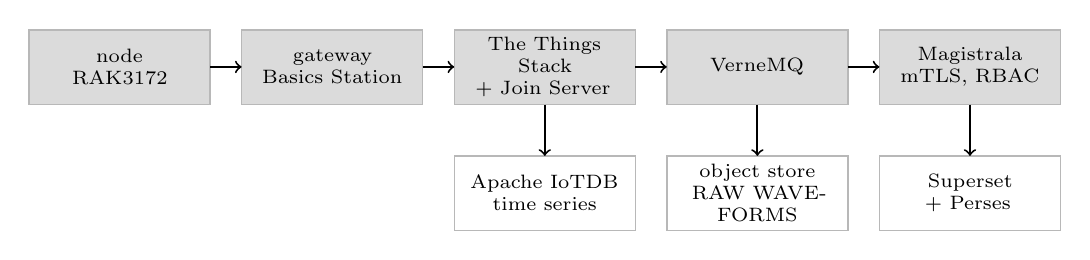
\begin{tikzpicture}[font=\scriptsize,node distance=0pt]
    \foreach \x/\y/\w/\l in {%
      0/0/2.3/{node\\RAK3172},
      2.7/0/2.3/{gateway\\Basics Station},
      5.4/0/2.3/{The Things Stack\\$+$ Join Server},
      8.1/0/2.3/{VerneMQ},
      10.8/0/2.3/{Magistrala\\mTLS, RBAC}}
      {\fill[fill1] (\x,\y) rectangle (\x+\w,\y+0.95);
       \draw[hair,line width=0.5pt] (\x,\y) rectangle (\x+\w,\y+0.95);
       \node[align=center,text width=2.1cm] at (\x+\w/2,\y+0.48) {\l};}
    \foreach \x in {2.3,5.0,7.7,10.4}
      {\draw[->,line width=0.7pt] (\x,0.48) -- (\x+0.4,0.48);}
    % second row
    \foreach \x/\l in {5.4/{Apache IoTDB\\time series},8.1/{object store\\RAW WAVEFORMS},10.8/{Superset\\$+$ Perses}}
      {\fill[fill0] (\x,-1.6) rectangle (\x+2.3,-0.65);
       \draw[hair,line width=0.5pt] (\x,-1.6) rectangle (\x+2.3,-0.65);
       \node[align=center,text width=2.1cm] at (\x+1.15,-1.12) {\l};}
    \foreach \x in {6.55,9.25,11.95}
      {\draw[->,line width=0.7pt] (\x,0.0) -- (\x,-0.65);}
  \end{tikzpicture}
  \vspace{0.7em}
  \begin{itemize}\footnotesize
    \item \textbf{\textasciitilde\$95--115/month} self-hosted at 10,000 devices. No Kubernetes, no
          Kafka, no ThingsBoard, no Grafana.
    \item \textbf{The highest-leverage spend above \$200/mo is not compute --- it is raw-waveform
          object storage.} Keep every waveform; the corpus is the input to everything.
    \item Spend the slack on managed Postgres for the Join Server: \textbf{losing LoRaWAN root key
          material is an extinction event}.
  \end{itemize}
\end{frame}

% ============================================================= 21
\begin{frame}{Certification critical path}
  \vspace{0.2em}
  \hspace*{\fill}%
  \begin{tikzpicture}[x=0.42cm,y=0.52cm,font=\tiny]
    % --- month grid, drawn first so everything sits on top of it
    \foreach \m in {0,...,24}
      {\draw[hair,line width=0.2pt] (\m,0.9) -- (\m,-5.9);}
    \foreach \m in {0,6,12,18,24}
      {\node[anchor=south,font=\tiny] at (\m,0.95) {\m};}
    \node[anchor=south,font=\scriptsize] at (12,1.6) {months};
    % --- phase boundaries
    \foreach \m/\p in {0/P0,1.5/P1,5/P2,12/P3}
      {\draw[ink,line width=0.7pt] (\m,0.9) -- (\m,-5.9);
       \node[anchor=north west,font=\tiny\bfseries] at (\m+0.15,-5.9) {\p};}
    % --- the two non-compressible items: full-width bars BEHIND everything else.
    %     This is the whole argument of the roadmap, made visual.
    \fill[fill1] (0,0.45) rectangle (24,-0.25);
    \draw[hair,line width=0.4pt] (0,0.45) rectangle (24,-0.25);
    \node[anchor=west,font=\tiny] at (0.3,0.1)
      {\textbf{One freeze/thaw cycle of labelled field data --- 12 months, cannot be bought}};
    \fill[fill1] (0,-0.55) rectangle (24,-1.25);
    \draw[hair,line width=0.4pt] (0,-0.55) rectangle (24,-1.25);
    \node[anchor=west,font=\tiny] at (0.3,-0.9)
      {\textbf{Insurer / aggregator procurement $+$ security review --- 6--18 months}};
    \node[anchor=east,font=\tiny,align=right,text width=3.1cm] at (-0.7,0.1) {\textbf{NOT COMPRESSIBLE}};
    \node[anchor=east,font=\tiny,align=right,text width=3.1cm] at (-0.7,-0.9) {\textbf{NOT COMPRESSIBLE}};
    % --- short bars inside (\gbar is defined in the preamble; see the comment there)
    \gbar{-1.9}{0.2}{1.5}{fill3}{\textbf{IAPMO scope letter \textperiodcentered{} CP}}
    \gbar{-2.5}{0.2}{2.2}{fill2}{FTO opinion}
    \gbar{-3.1}{0.5}{1.5}{fill2}{20-valve spike}
    \gbar{-3.7}{1.5}{5.0}{fill2}{E\&O bound \textperiodcentered{} SOC 2 Type I}
    \gbar{-4.3}{5.0}{7.0}{fill2}{module MOQ 8--20 wk}
    \gbar{-4.9}{7.0}{9.5}{fill3}{\textbf{FCC lab queue $+$ test \textperiodcentered{} CP}}
    \gbar{-5.5}{8.0}{11.0}{fill2}{tooling $+$ 2--3 iterations}
    % dependency: grant must land before tooling commits
    \draw[->,line width=0.5pt] (9.5,-4.9) -- (9.5,-5.22);
  \end{tikzpicture}%
  \hspace*{\fill}
  \vspace{0.4em}
  \par
  {\raggedright\scriptsize \textbf{CP} $=$ critical path (darkest fill). The two
   \textsc{not compressible} bars span the whole chart; FCC and tooling are \emph{short bars inside
   them}. That is the argument of the entire roadmap in one picture:
   \textbf{hardware is not the critical path} --- it only has to not be late.\par}
\end{frame}

% ============================================================= 22
\begin{frame}{Can we dodge the plumbing standards?}
  \scriptsize
  \begin{tabular}{@{}p{0.20\textwidth}p{0.34\textwidth}p{0.38\textwidth}@{}}
    \toprule
    \hd{Standard} & \hd{Scope} & \hd{Retrofit lever actuator} \\
    \midrule
    NSF/ANSI 61 & what leaches into drinking water & \cellcolor{fill1}\textbf{Out} --- no wetted surface \\
    NSF/ANSI 372 & $\leq$0.25\% lead on potable-contact surfaces & \cellcolor{fill1}\textbf{Out} --- no wetted surface \\
    IAPMO IGC 115/349 & automatic leak detection / supply-integrity devices & \textbf{Probably out} --- no pressure boundary, so most of the test matrix is physically inapplicable. \emph{Get it in writing} \\
    UL 498 / 60730-1 & mains-powered devices & \cellcolor{fill1}\textbf{Out} if battery or an externally supplied listed adapter \\
    \bottomrule
  \end{tabular}
  \vspace{0.6em}
  \begin{itemize}\footnotesize
    \item \textbf{ASSE 1087 is the wrong document} --- it is commercial/food-service water
          \emph{treatment} equipment. The IGC numbers above are the real ones.
    \item \textbf{Hard BOM rule: actuator only, no plumbing parts in the box.} One adapter and the
          kit becomes a plumbing product.
    \item The blocker is mechanical: breakaway torque on aged valves, \textbf{stem weep after years
          of set packing}, and \textbf{multi-turn gate valves that a quarter-turn actuator cannot
          drive at all}.
  \end{itemize}
  \vspace{0.2em}
  \gate{\textbf{$>$70\% of twenty salvaged aged valves cycle without stem weep.} Cost: a few hundred
        dollars. Fail $\rightarrow$ kill option B permanently and resell a certified valve.}
\end{frame}

% ============================================================= 23
\begin{frame}{Risk register, top 12}
  \scriptsize
  \begin{tabular}{@{}p{0.01\textwidth}p{0.27\textwidth}cc p{0.22\textwidth}p{0.29\textwidth}@{}}
    \toprule
    & \hd{Risk} & \hd{L} & \hd{I} & \hd{Leading indicator} & \hd{Mitigation} \\
    \midrule
    1&\textbf{No buyer signs with a pre-seed vendor} & H & \cellcolor{fill3}\textbf{fatal} & no countersigned doc by wk 6 & route via MGA/aggregator; run all 4 routes \\
    2&False positives destroy insurer trust & H & H & nuisance rate not falling wk/wk & shadow mode; install-verify telemetry \\
    3&Loss reduction unprovable at this scale & H & H & pilot $<$2{,}000 house-years & \textbf{agree a surrogate metric in P0} \\
    4&Install-quality failure tail & H & M & $>$10\% never reporting at day 7 & don't count unverified installs \\
    5&LoRaWAN downlink unreliable for shutoff & H & H & any doc with cloud closing the valve & \textbf{architectural: decide locally} \\
    6&Premium credit unfilable / anti-rebating & M & \cellcolor{fill3}\textbf{fatal} & counsel won't commit to a filing path & \textbf{sell loss control, not a discount} \\
    7&Battery life in a cold basement & H & M & pulse behaviour at $-10$ to $0^{\circ}$C & Li-SOCl\textsubscript{2} $+$ HLC; derate 40\%; measure \\
    8&Module EOL invalidates the FCC grant & M & H & vendor PCN; lead time $>$16 wk & same-vendor alternate; budget the re-test \\
    9&Valve fails closed (or silently open) & M & H & any unit arming above torque threshold & refuse to arm; \textbf{fail-as-is}; override \\
    10&The data moat is not defensible & M & H & model flat per 1k device-months & own the relationship; fix data rights in contract \\
    11&ODM dependency / landed-cost swing & M & M & landed cost moving $>$15\% & own firmware $+$ fixtures; dual-quote a NA CM \\
    12&\textbf{Seasonality makes slip non-linear} & M & H & devices not in field by October & \textbf{a 6-week slip costs 12 months} \\
    \bottomrule
  \end{tabular}
  \vspace{0.4em}
  {\scriptsize\color{inkmute} Likelihood and impact are text tokens, sorted by L$\times$I ---
   deliberately not colour-coded, because red and green are \textasciitilde1.3:1 apart in greyscale.\par}
\end{frame}

% ============================================================= 24
\begin{frame}{First 90 days, and what we will not build}
  \begin{columns}[t]
  \begin{column}{0.49\textwidth}
    {\footnotesize\textbf{The first 90 days}}
    \begin{itemize}\scriptsize
      \item \textbf{Wk 1:} lock the \emph{module ecosystem} (not the radio); send the \textbf{IAPMO
            scope letter}; ingest live with raw retention.
      \item \textbf{Wk 1--2:} commission the \textbf{FTO opinion}.
      \item \textbf{Wk 2--6:} \textbf{20--30 dev-kit nodes into 10--20 real buildings}.
      \item \textbf{Wk 2--12:} \textbf{25 buyer conversations, all four routes} --- target one
            countersigned document.
      \item \textbf{Wk 6--12:} the \textbf{20-valve spike}; bind E\&O; start SOC 2 readiness.
      \item \textbf{Throughout: no PCB layout. No Gerbers exist.}
    \end{itemize}
  \end{column}
  \begin{column}{0.49\textwidth}
    {\footnotesize\textbf{What we will not build}}
    \begin{itemize}\scriptsize
      \item No inline valve in year 1 --- resell a certified one.
      \item No mains-powered product in year 1.
      \item \textbf{No arc-fault interruption, ever} --- that is UL 1699 at $+$\$60--200k. Alert
            only, like Ting.
      \item No own device-management or OTA backend.
      \item No neural network on the node before P2.
      \item No FUOTA over LoRaWAN; no own network server under 1{,}000 nodes.
      \item No Matter before a DTC buyer exists.
      \item \textbf{No AGPL or GPL in the product path.}
      \item No custom gateway hardware --- RAK sells them from \$99.
      \item No premium-share or MGA structure in year 1.
    \end{itemize}
  \end{column}
  \end{columns}
  \vspace{0.3em}
  \gate{P0: a countersigned paid pilot or LOI for $\geq$50 units \emph{with a start date}.}
\end{frame}

% ============================================================= appendix
\appendix
\begin{frame}{Appendix A --- indicative BOM, clamp-on sensor}
  \scriptsize
  \begin{tabular}{@{}p{0.42\textwidth}p{0.26\textwidth}rp{0.14\textwidth}@{}}
    \toprule
    \hd{Item} & \hd{Part} & \hd{\$ @1k} & \hd{Evidence} \\
    \midrule
    Radio $+$ MCU module          & RAK3172 (STM32WLE5) & 5.99 & [V] \\
    \quad alternate, adds BLE     & RAK11720            & 7.99 & [V] \\
    \quad second source           & Seeed Wio-E5        & 6.49 & [V] \\
    Pipe temperature              & TI TMP117           & 3.62 & [V] \\
    Ambient temperature           & TI TMP117           & 3.62 & [V] \\
    Tamper/sanity channel         & NTC                 & 0.15 & [E] \\
    Battery                       & 2$\times$ Li-SOCl\textsubscript{2} AA & 5.00 & [E] \\
    Pulse support                 & hybrid-layer cap    & 1.20 & [E] \\
    Antenna                       & chip/wire 915\,MHz  & 0.45 & [E] \\
    PCB $+$ assembly              & 4-layer 40$\times$60\,mm & 3.50 & [E] \\
    Enclosure, clip, thermal pad  & moulded ABS/PC      & 4.00 & [E] \\
    \midrule
    \textbf{Total}                &                     & \textbf{\textasciitilde27} & mid-point \\
    \bottomrule
  \end{tabular}
  \vspace{0.5em}
  {\scriptsize Excludes amortised tooling, freight, duty and test. Full file:
   \texttt{data/bom-estimates.csv}.\par}
\end{frame}

\begin{frame}{Appendix B --- certification line items}
  \scriptsize
  \begin{tabular}{@{}p{0.46\textwidth}rrp{0.18\textwidth}@{}}
    \toprule
    \hd{Line (clamp-on sensor)} & \hd{Low} & \hd{High} & \hd{Evidence} \\
    \midrule
    FCC/ISED composite, module grant inherited & 1{,}500 & 5{,}000 & [E] \\
    LoRa Alliance membership (startup rate)    & 3{,}000 & 6{,}000 & [V] \\
    LoRaWAN cert, end device at an ATL         & 1{,}200 & 1{,}700 & [V] \\
    Plumbing listing                           & 0 & 0 & verified \\
    NRTL safety listing                        & 0 & 0 & verified \\
    Tooling, EVT/DVT, FTO opinion              & 25{,}000 & 80{,}000 & [E] \\
    \midrule
    \textbf{Total to shippable}                & \textbf{\textasciitilde31k} & \textbf{\textasciitilde94k} & \\
    \bottomrule
  \end{tabular}
  \vspace{0.7em}
  \begin{itemize}\scriptsize
    \item Plug-in detector: \textbf{\$180--560k} --- NRTL \$15--40k, classifier \$150--500k,
          $+$\$60--200k if it ever interrupts.
    \item Inline valve: \textbf{\$112--366k} --- IGC $+$ NSF $+$ cUPC $+$ UL 60730.
    \item \textbf{OSHA recognises 21 NRTLs.} Get three quotes --- Intertek ETL and QPS routinely
          undercut UL. NSF and IAPMO EGS are themselves NRTLs, so one body can scope both.
  \end{itemize}
\end{frame}

\begin{frame}{Appendix C --- gateway economics}
  \scriptsize
  \begin{tabular}{@{}p{0.34\textwidth}p{0.30\textwidth}r@{}}
    \toprule
    \hd{Deployment} & \hd{Gateway} & \hd{\$ [V]} \\
    \midrule
    Single home, customer internet      & RAK7266 Soho Lite      & 99 \\
    Single home, better radio           & RAK7268V2 Edge Lite 2  & 154 \\
    \textbf{Unreliable/absent internet} & \textbf{RAK7268CV2-V (Verizon)} & \textbf{299} \\
    \textbf{Multi-dwelling}             & \textbf{RAK7289V2 Edge Pro}     & \textbf{382} \\
    Campus / outdoor                    & RAK7285 / RAK7393      & 799 / 439 \\
    \bottomrule
  \end{tabular}
  \vspace{0.7em}
  \begin{tabular}{@{}p{0.34\textwidth}rr@{}}
    \toprule
    & \hd{Single-family} & \hd{40-unit building} \\
    \midrule
    Gateway                        & \$99--299 & \$382 \\
    Nodes                          & 1 $\times$ \$27 & 40 $\times$ \$12 $=$ \$480 \\
    \textbf{Gateway as \% of HW}   & \cellcolor{fill2}\textbf{79--92\%} & \cellcolor{fill1}\textbf{44\%} \\
    \bottomrule
  \end{tabular}
  \vspace{0.6em}
  \begin{itemize}\scriptsize
    \item \textbf{In a single-family home the gateway costs 3--10$\times$ the sensor.} That kills a
          consumer price point and is dead weight in an insurer-funded BOM.
    \item So if you ship a gateway per home anyway, \textbf{ask what LoRa is buying you} --- BLE or
          LTE-M does it more cheaply. \textbf{LoRaWAN's economics live in buildings.}
    \item The \$299 Verizon unit is the exception worth considering: it removes the homeowner's
          router from your support burden, and support cost often exceeds the \$145 delta.
  \end{itemize}
\end{frame}

\begin{frame}{Appendix D --- public LoRaWAN coverage reality}
  \footnotesize
  \begin{itemize}
    \item \textbf{Senet no longer exists independently} --- redirects to Netmore, which
          \textbf{acquired Actility in January 2026}. Two of three names in the original brief are
          now one vendor.
    \item \textbf{Everynet} fails its TLS handshake. \textbf{Helium} has pivoted cellular-first.
    \item \textbf{TTN:} 249{,}612 members, but \textasciitilde43 forum posts in the last 7 days.
    \item \textbf{Amazon Sidewalk} is the dark horse --- the only 900\,MHz network whose gateways
          (Echo, Ring) are \emph{already inside American homes}. Severe payload limits; total Amazon
          dependency.
  \end{itemize}
  \vspace{0.5em}
  \begin{beamercolorbox}[wd=\textwidth,sep=1.6ex]{}
    \color{ink}\small The decisive argument is \textbf{operational, not coverage}: \textbf{no US
    operator gives you an API to pre-qualify a customer's address before you ship them a box.}
    A hardware company shipping devices that might not connect has an unmanageable returns cost.
  \end{beamercolorbox}
  \vspace{0.5em}
  {\scriptsize\color{inkmute} Also dead: \textbf{Arm Mbed OS reached EOL in July 2026}
   (\texttt{os.mbed.com} now redirects to GitHub) \textperiodcentered{} ESP-IDF v5.2 branch EOL
   August 2026 \textperiodcentered{} TI AMC130M03 has no distributor stock anywhere.\par}
\end{frame}

\end{document}
